\section{Referencia de la Clase Albaran\-Cliente}
\label{classAlbaranCliente}\index{AlbaranCliente@{AlbaranCliente}}
Clase que almacena los datos de albaranes a clientes.  


{\tt \#include $<$albarancliente.h$>$}

Diagrama de herencias de Albaran\-Cliente\begin{figure}[H]
\begin{center}
\leavevmode
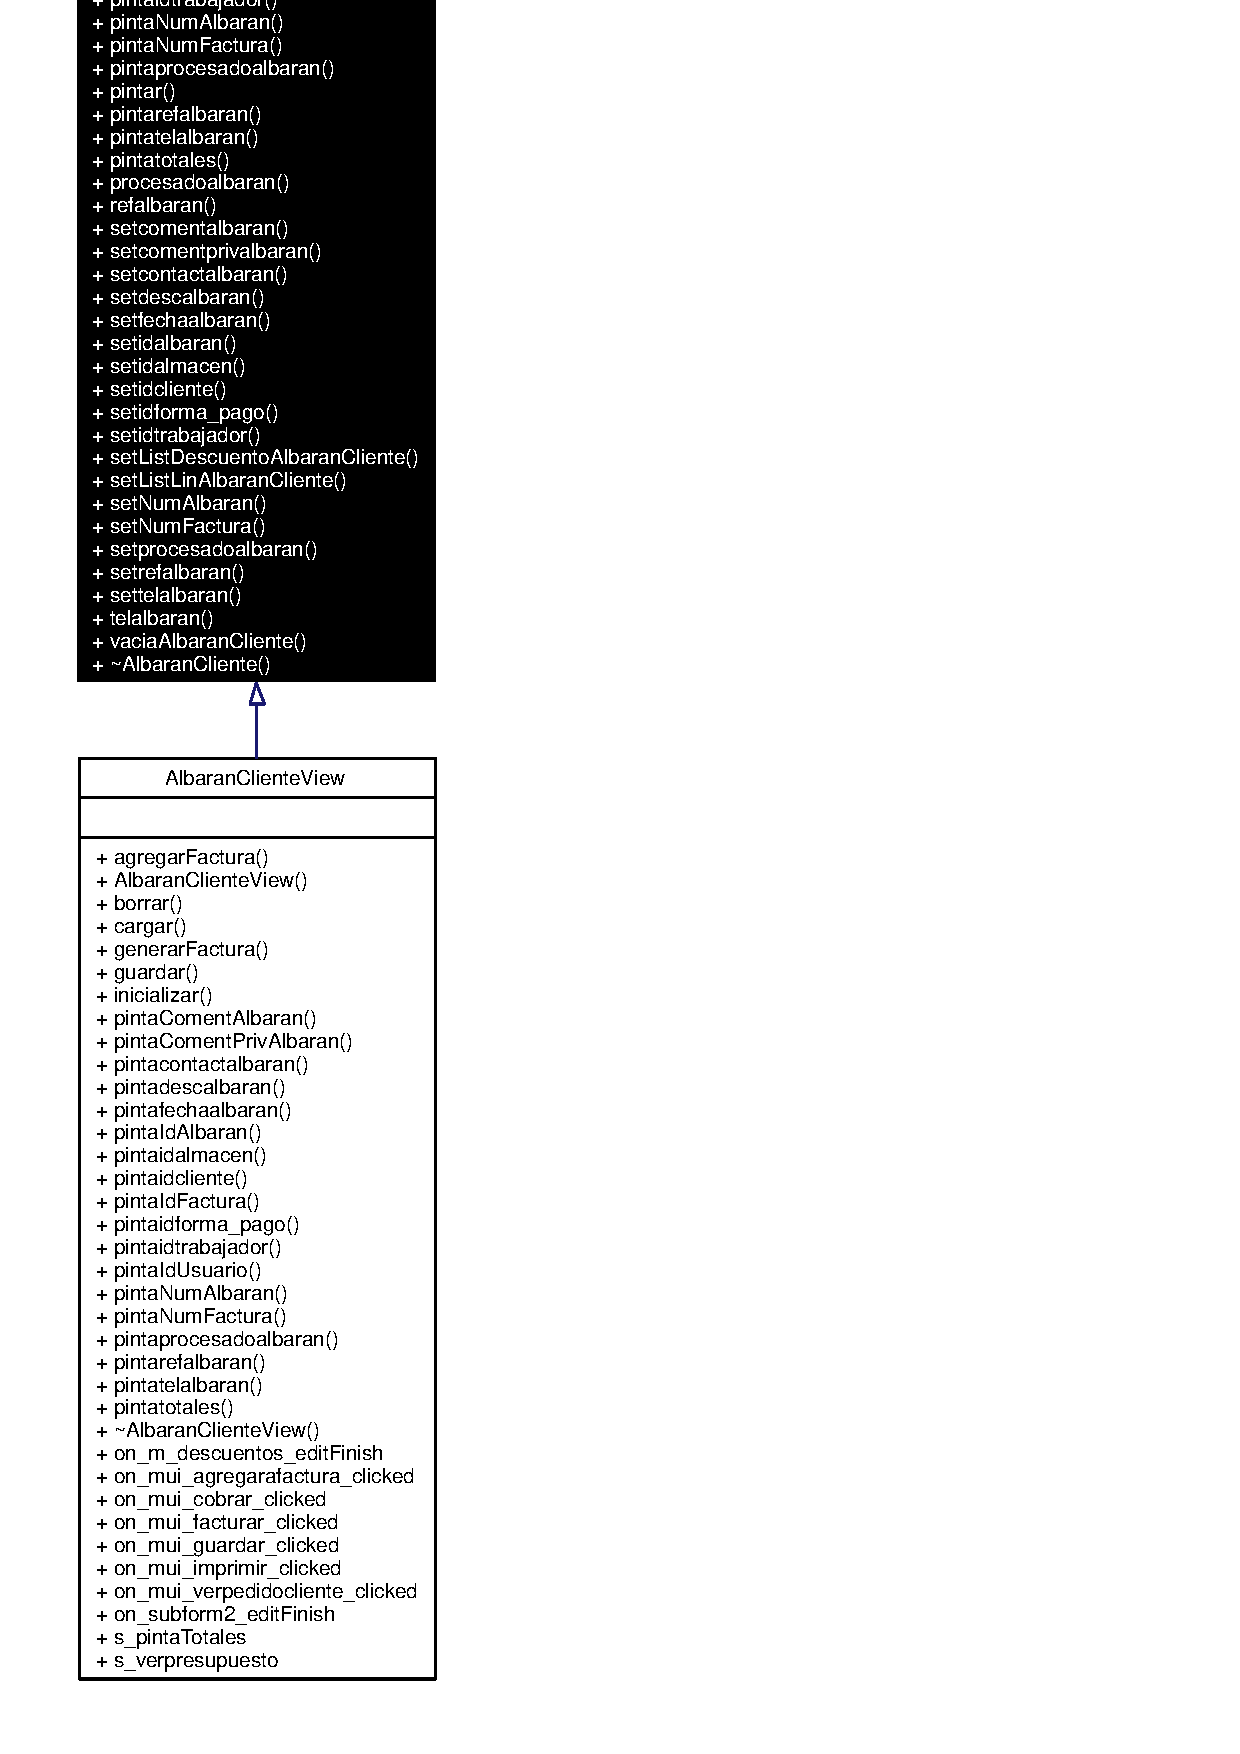
\includegraphics[width=105pt]{classAlbaranCliente__inherit__graph}
\end{center}
\end{figure}
Diagrama de colaboraci\'{o}n para Albaran\-Cliente:\begin{figure}[H]
\begin{center}
\leavevmode
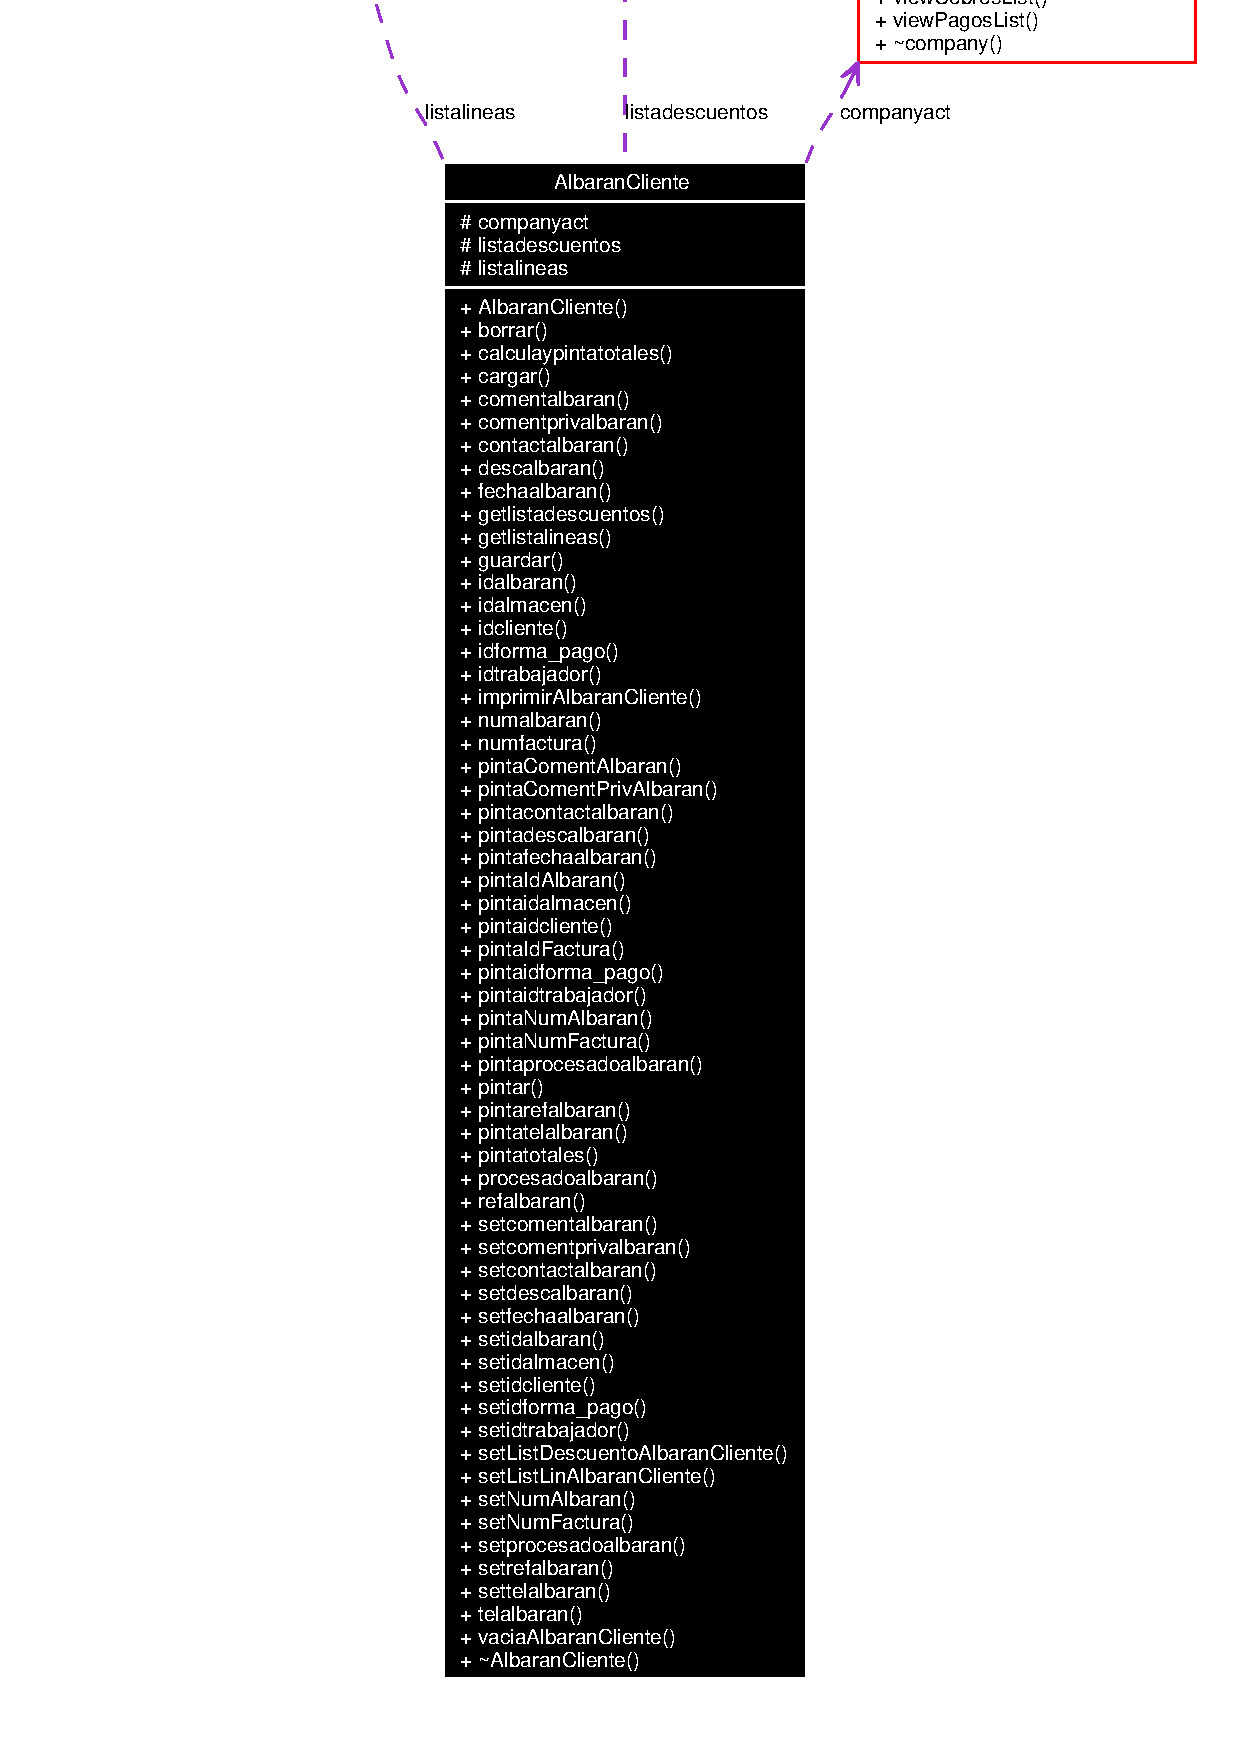
\includegraphics[width=287pt]{classAlbaranCliente__coll__graph}
\end{center}
\end{figure}
\subsection*{M\'{e}todos p\'{u}blicos}
\begin{CompactItemize}
\item 
{\bf Albaran\-Cliente} ({\bf company} $\ast$)\label{classAlbaranCliente_a0}

\item 
virtual int {\bf borrar} ()\label{classAlbaranCliente_a1}

\item 
virtual void {\bf calculaypintatotales} ()
\item 
virtual int {\bf cargar} (QString)\label{classAlbaranCliente_a3}

\begin{CompactList}\small\item\em Esta funcioncarga un Albaran\-Cliente. \item\end{CompactList}\item 
QString {\bf comentalbaran} ()\label{classAlbaranCliente_a4}

\item 
QString {\bf comentprivalbaran} ()\label{classAlbaranCliente_a5}

\item 
QString {\bf contactalbaran} ()\label{classAlbaranCliente_a6}

\item 
QString {\bf descalbaran} ()\label{classAlbaranCliente_a7}

\item 
QString {\bf fechaalbaran} ()\label{classAlbaranCliente_a8}

\item 
{\bf List\-Descuento\-Albaran\-Cliente\-View} $\ast$ {\bf getlistadescuentos} ()\label{classAlbaranCliente_a9}

\item 
{\bf List\-Lin\-Albaran\-Cliente\-View} $\ast$ {\bf getlistalineas} ()\label{classAlbaranCliente_a10}

\item 
virtual int {\bf guardar} ()
\item 
QString {\bf idalbaran} ()\label{classAlbaranCliente_a12}

\item 
QString {\bf idalmacen} ()\label{classAlbaranCliente_a13}

\item 
QString {\bf idcliente} ()\label{classAlbaranCliente_a14}

\item 
QString {\bf idforma\_\-pago} ()\label{classAlbaranCliente_a15}

\item 
QString {\bf idtrabajador} ()\label{classAlbaranCliente_a16}

\item 
void {\bf imprimir\-Albaran\-Cliente} ()
\item 
QString {\bf numalbaran} ()\label{classAlbaranCliente_a18}

\item 
QString {\bf numfactura} ()\label{classAlbaranCliente_a19}

\item 
virtual void {\bf pinta\-Coment\-Albaran} (QString)\label{classAlbaranCliente_a20}

\item 
virtual void {\bf pinta\-Coment\-Priv\-Albaran} (QString)\label{classAlbaranCliente_a21}

\item 
virtual void {\bf pintacontactalbaran} (QString)\label{classAlbaranCliente_a22}

\item 
virtual void {\bf pintadescalbaran} (QString)\label{classAlbaranCliente_a23}

\item 
virtual void {\bf pintafechaalbaran} (QString)\label{classAlbaranCliente_a24}

\item 
virtual void {\bf pinta\-Id\-Albaran} (QString)\label{classAlbaranCliente_a25}

\item 
virtual void {\bf pintaidalmacen} (QString)\label{classAlbaranCliente_a26}

\item 
virtual void {\bf pintaidcliente} (QString)\label{classAlbaranCliente_a27}

\item 
virtual void {\bf pinta\-Id\-Factura} (QString)\label{classAlbaranCliente_a28}

\item 
virtual void {\bf pintaidforma\_\-pago} (QString)\label{classAlbaranCliente_a29}

\item 
virtual void {\bf pintaidtrabajador} (QString)\label{classAlbaranCliente_a30}

\item 
virtual void {\bf pinta\-Num\-Albaran} (QString)\label{classAlbaranCliente_a31}

\item 
virtual void {\bf pinta\-Num\-Factura} (QString)\label{classAlbaranCliente_a32}

\item 
virtual void {\bf pintaprocesadoalbaran} (QString)\label{classAlbaranCliente_a33}

\item 
virtual void {\bf pintar} ()
\item 
virtual void {\bf pintarefalbaran} (QString)\label{classAlbaranCliente_a35}

\item 
virtual void {\bf pintatelalbaran} (QString)\label{classAlbaranCliente_a36}

\item 
virtual void {\bf pintatotales} (Fixed, Fixed, Fixed, Fixed)\label{classAlbaranCliente_a37}

\item 
QString {\bf procesadoalbaran} ()\label{classAlbaranCliente_a38}

\item 
QString {\bf refalbaran} ()\label{classAlbaranCliente_a39}

\item 
void {\bf setcomentalbaran} (QString val)\label{classAlbaranCliente_a40}

\item 
void {\bf setcomentprivalbaran} (QString val)\label{classAlbaranCliente_a41}

\item 
void {\bf setcontactalbaran} (QString val)\label{classAlbaranCliente_a42}

\item 
void {\bf setdescalbaran} (QString val)\label{classAlbaranCliente_a43}

\item 
void {\bf setfechaalbaran} (QString val)\label{classAlbaranCliente_a44}

\item 
void {\bf setidalbaran} (QString val)\label{classAlbaranCliente_a45}

\item 
void {\bf setidalmacen} (QString val)\label{classAlbaranCliente_a46}

\item 
void {\bf setidcliente} (QString val)\label{classAlbaranCliente_a47}

\item 
void {\bf setidforma\_\-pago} (QString val)\label{classAlbaranCliente_a48}

\item 
void {\bf setidtrabajador} (QString val)\label{classAlbaranCliente_a49}

\item 
void {\bf set\-List\-Descuento\-Albaran\-Cliente} ({\bf List\-Descuento\-Albaran\-Cliente\-View} $\ast$a)\label{classAlbaranCliente_a50}

\item 
void {\bf set\-List\-Lin\-Albaran\-Cliente} ({\bf List\-Lin\-Albaran\-Cliente\-View} $\ast$a)
\item 
void {\bf set\-Num\-Albaran} (QString val)\label{classAlbaranCliente_a52}

\item 
void {\bf set\-Num\-Factura} (QString val)\label{classAlbaranCliente_a53}

\item 
void {\bf setprocesadoalbaran} (QString val)\label{classAlbaranCliente_a54}

\item 
void {\bf setrefalbaran} (QString val)\label{classAlbaranCliente_a55}

\item 
void {\bf settelalbaran} (QString val)\label{classAlbaranCliente_a56}

\item 
QString {\bf telalbaran} ()\label{classAlbaranCliente_a57}

\item 
void {\bf vacia\-Albaran\-Cliente} ()\label{classAlbaranCliente_a58}

\end{CompactItemize}
\subsection*{Atributos protegidos}
\begin{CompactItemize}
\item 
{\bf company} $\ast$ {\bf companyact}\label{classAlbaranCliente_p0}

\item 
{\bf List\-Descuento\-Albaran\-Cliente\-View} $\ast$ {\bf listadescuentos}\label{classAlbaranCliente_p1}

\item 
{\bf List\-Lin\-Albaran\-Cliente\-View} $\ast$ {\bf listalineas}\label{classAlbaranCliente_p2}

\end{CompactItemize}


\subsection{Descripci\'{o}n detallada}
Clase que almacena los datos de albaranes a clientes. 



\subsection{Documentaci\'{o}n de las funciones miembro}
\index{AlbaranCliente@{Albaran\-Cliente}!calculaypintatotales@{calculaypintatotales}}
\index{calculaypintatotales@{calculaypintatotales}!AlbaranCliente@{Albaran\-Cliente}}
\subsubsection{\setlength{\rightskip}{0pt plus 5cm}void Albaran\-Cliente::calculaypintatotales ()\hspace{0.3cm}{\tt  [virtual]}}\label{classAlbaranCliente_a2}


Impresion de los contenidos.

Impresion de los descuentos. \index{AlbaranCliente@{Albaran\-Cliente}!guardar@{guardar}}
\index{guardar@{guardar}!AlbaranCliente@{Albaran\-Cliente}}
\subsubsection{\setlength{\rightskip}{0pt plus 5cm}int Albaran\-Cliente::guardar ()\hspace{0.3cm}{\tt  [virtual]}}\label{classAlbaranCliente_a11}


Todo el guardado es una transaccion. 

Reimplementado en {\bf Albaran\-Cliente\-View} {\rm (p.\,\pageref{classAlbaranClienteView_a5})}.\index{AlbaranCliente@{Albaran\-Cliente}!imprimirAlbaranCliente@{imprimirAlbaranCliente}}
\index{imprimirAlbaranCliente@{imprimirAlbaranCliente}!AlbaranCliente@{Albaran\-Cliente}}
\subsubsection{\setlength{\rightskip}{0pt plus 5cm}void Albaran\-Cliente::imprimir\-Albaran\-Cliente ()}\label{classAlbaranCliente_a17}


Copiamos el archivo.

Copiamos el logo.

Linea de totales del presupuesto.

Impresion de la tabla de contenidos.

Impresion de los descuentos.

Impresi\~{A}179n de los totales.

Rellena el primer tr de titulares.

Rellena el segundo tr de cantidades. \index{AlbaranCliente@{Albaran\-Cliente}!pintar@{pintar}}
\index{pintar@{pintar}!AlbaranCliente@{Albaran\-Cliente}}
\subsubsection{\setlength{\rightskip}{0pt plus 5cm}void Albaran\-Cliente::pintar ()\hspace{0.3cm}{\tt  [virtual]}}\label{classAlbaranCliente_a34}


Pinta el subformulario de detalle del Albaran\-Cliente. Pintamos los totales. \index{AlbaranCliente@{Albaran\-Cliente}!setListLinAlbaranCliente@{setListLinAlbaranCliente}}
\index{setListLinAlbaranCliente@{setListLinAlbaranCliente}!AlbaranCliente@{Albaran\-Cliente}}
\subsubsection{\setlength{\rightskip}{0pt plus 5cm}void Albaran\-Cliente::set\-List\-Lin\-Albaran\-Cliente ({\bf List\-Lin\-Albaran\-Cliente\-View} $\ast$ {\em a})\hspace{0.3cm}{\tt  [inline]}}\label{classAlbaranCliente_a51}


Establece cual es la lista subformulario del presupuesto. Normalmente para apuntar a listlinpresupuestoview. 

La documentaci\'{o}n para esta clase fu\'{e} generada a partir de los siguientes archivos:\begin{CompactItemize}
\item 
albarancliente.h\item 
albarancliente.cpp\end{CompactItemize}
